\begin{figure}[t]
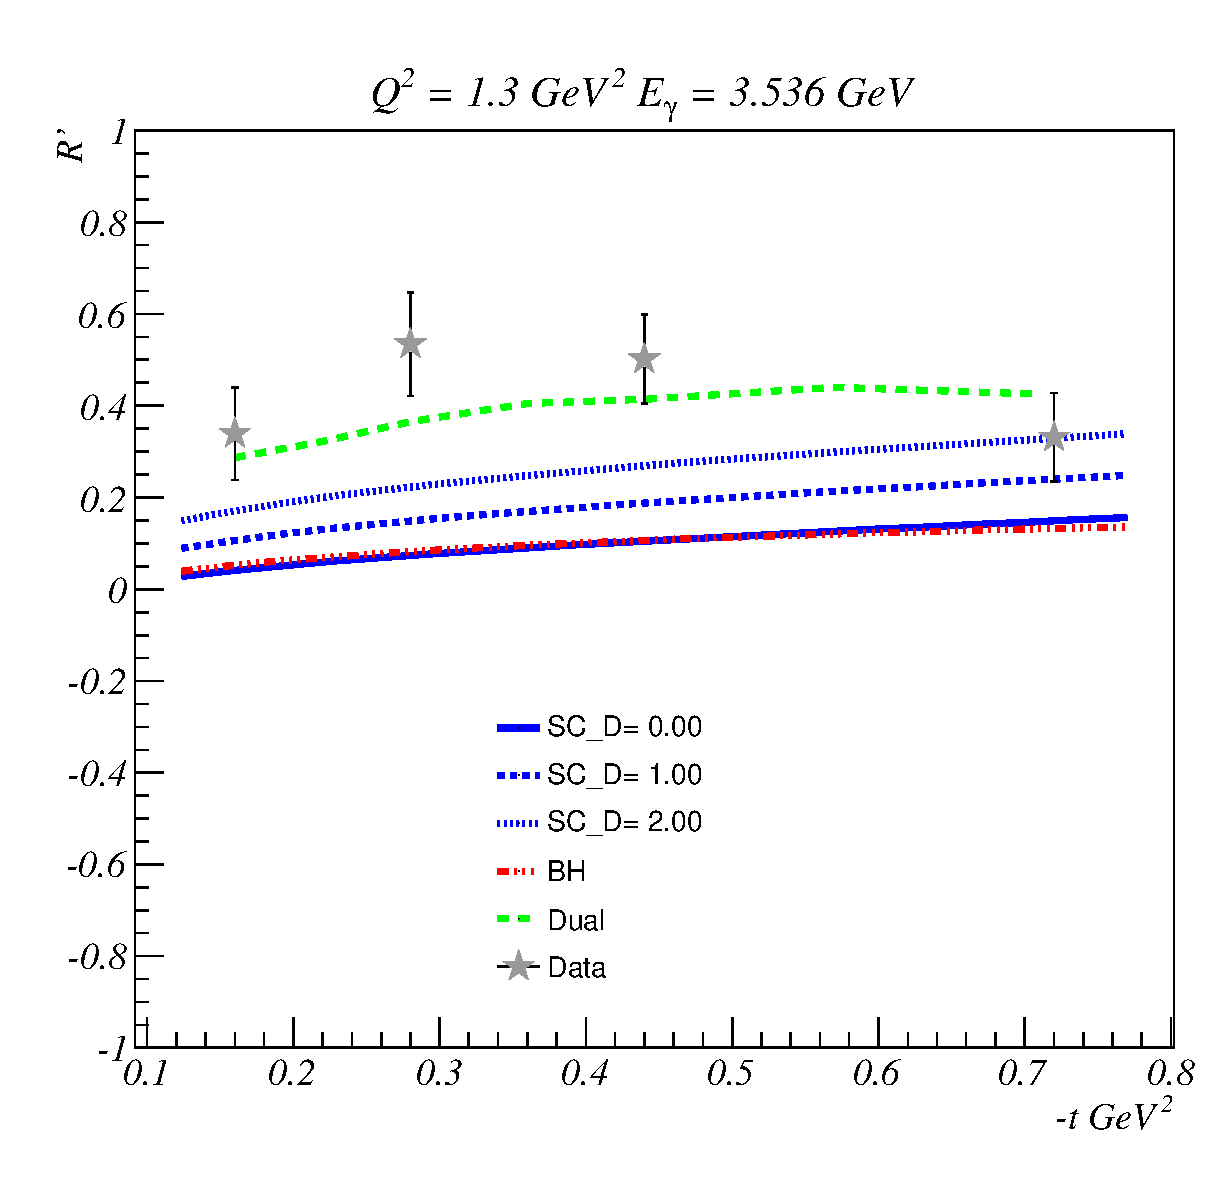
\includegraphics[scale=0.45]{R_dep_theta_var_6GeV.eps}
\caption{\small{The cosine moment of the weighted cross section, $R'$, in
the CLAS acceptance compared to GPD model calculations based on the dual
parametrization
\cite{Polyakov:2002wz,Guzey:2006xi,Guzey:2008ys,Polyakov:2008aa}
(upper, green curve), and the double distribution
\cite{Radyushkin:1998es} (lower, blue curves) for three weights applied
to the $D$-term. The BH-contribution is shown in red.}}
\label{fig:R_dep_theta_var_6GeV}
\end{figure}

Our proposed SoLID experiment builds upon experience gained from the analysis
of CLAS 6 GeV data, which has established the technique for carrying
out exclusive photoproduction experiments with quasi-real photons that we
propose for this experiment with SoLID. As will be discussed in Sec.
\ref{sec:tcs_selection}, this requires the detection of all final-state
particles except the scattered electron, for which the missing mass and
missing transverse momentum are constrained to be very small.
More specifically, this technique has also been successfully applied to pilot
measurements of timelike Compton scattering using the CLAS e1-6 and e1f data
sets. The results from this CLAS Approved Analysis (CAA-DP09-01) have been
documented in Ref.~\cite{Rafael:2010}. It demonstrated an impressive pion
pair rejection of factor of $2.07 \times 10^{-7}$. Measuring the $\phi$ cross
section in parallel with TCS showed that the flux of quasi-real photons is
well understood.
The results from the above analysis could also be compared with an TCS
analysis using the g12 data set, which was the only high-energy CLAS data set
with tagged real photons (up to 5.7 GeV) that utilized the Cherenkov counters.
These had been made ready specifically for TCS and other $e^+e^-$ physics. The
analysis of the g12 data is still ongoing, but preliminary results seems to be
in line with what was obtained with the quasi-real photon technique.
The tagged-photon beam will also make it possible to do an independent
determination of the photon flux, and offer an opportunity to explore event
topologies with only two out of the three final-state particles detected.

In addition to demonstrating the feasibility of the proposed measurement, the
pilot experiments at 6 GeV stimulated the development of new analysis methods.
An example of this was the introduction of the cosine moment $R'$, evaluated
within the acceptance of the detector in the $\varphi_{CM}-\theta_{CM}$ plane
(the lepton c.m. angles $\varphi$ and $\theta$ are defined in
Fig.~\ref{fig:Angle}). Whereas the original definition of $R$ implies using
the integration ranges shown in Eqs.(\ref{eq:S}) and (\ref{eq:R}), $R'$ adds
an function $a(\theta_{CM},\varphi_{CM})$ corresponding to the detector
acceptance for a given kinematic bin. Utilizing the same acceptance function
for both the experimental and theoretical evaluations allows a straightforward
comparison between data and predictions based on various GPD models. The
difference between $R'$ and $R$ is discussed in more detail in
Sec. \ref{sec:tcsrate} together with the projected results.

Fig.~\ref{fig:R_dep_theta_var_6GeV} shows $R'$ extracted from the combined
e1-6 and e1f data sets for four bins in $-t$, compared with two GPD model
calculations based on the dual parametrization
\cite{Polyakov:2002wz,Guzey:2006xi,Guzey:2008ys,Polyakov:2008aa} and double
distribution \cite{Radyushkin:1998es}, respectively. Results from the latter
are shown with three weights for the contribution from the $D$-term (0, 1, and
2). Both the experimental and theoretical points shown here were evaluated at
the average value for the bin, but an event-by-event approach will be adopted
in the future.

\begin{figure}[t]
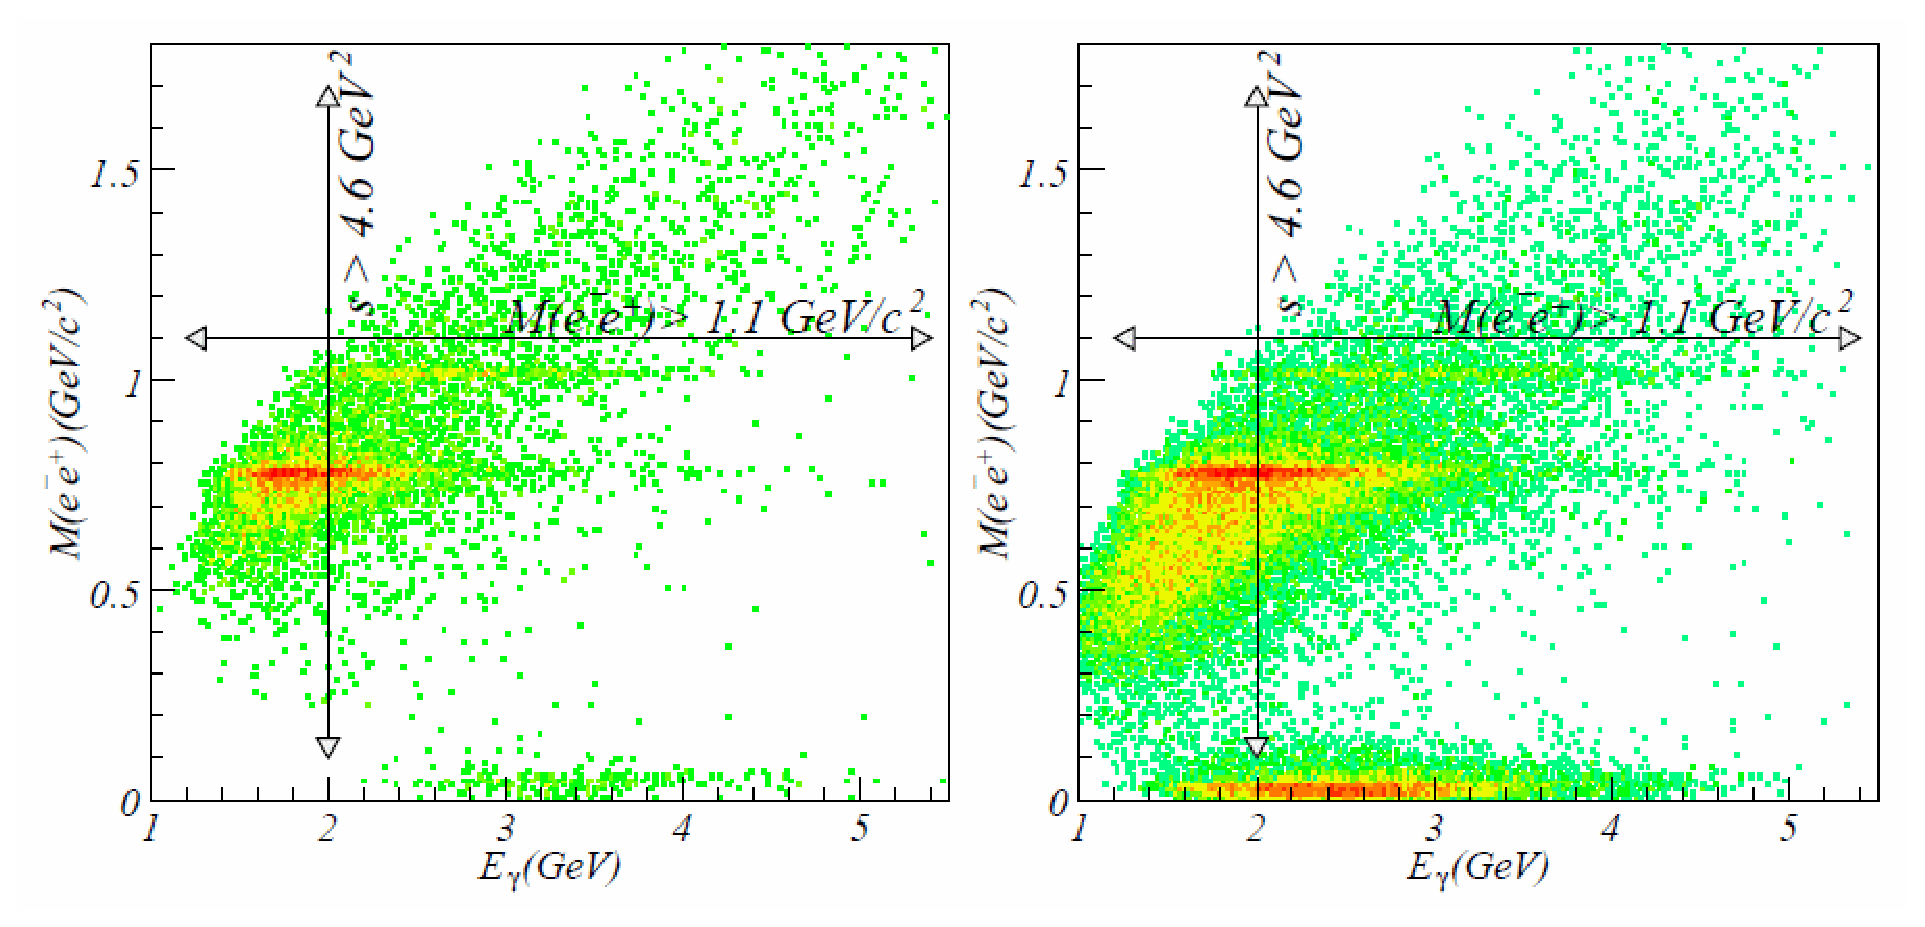
\includegraphics[scale=0.45]{TCS407.eps}
\caption{\small{$e^+e^-$ invariant mass vs. quasi-real photon energy for the
e1-6 (left) and e1f (right) data sets. Only events with $M_{ee}$ above the
$\phi$ mass were used for TCS analysis at 6 GeV.}}
\label{fig:TCS6}
\end{figure}

However, despite the usefulness of the 6 GeV data for developing the TCS
program, only the 12 GeV era will provide the required luminosity and
kinematic coverage. In particular, the higher beam energy will make it
possible to study a range of invariant lepton pair masses where there are no
meson resonances that complicate the interpretation of the measurement. As
shown in Fig.~\ref{fig:TCS6}, only data above the $\phi$ mass were used for
TCS analysis at 6 GeV, but at 12 GeV it will be possible to move this range
above the mass of the $\rho^{\prime}$.
%as shown in Fig. \ref{fig:ee_to_hadrons}.
